\documentclass[tikz,border=4pt]{standalone}
\usepackage{amsmath,amssymb}
\usepackage{tikz,pgfplots}
\pgfplotsset{compat=1.18}
\usetikzlibrary{arrows.meta,calc,positioning}
\begin{document}
% Generated from the archived contact-error endpoint summary.
% Values are means with sample standard deviations over three repetitions.
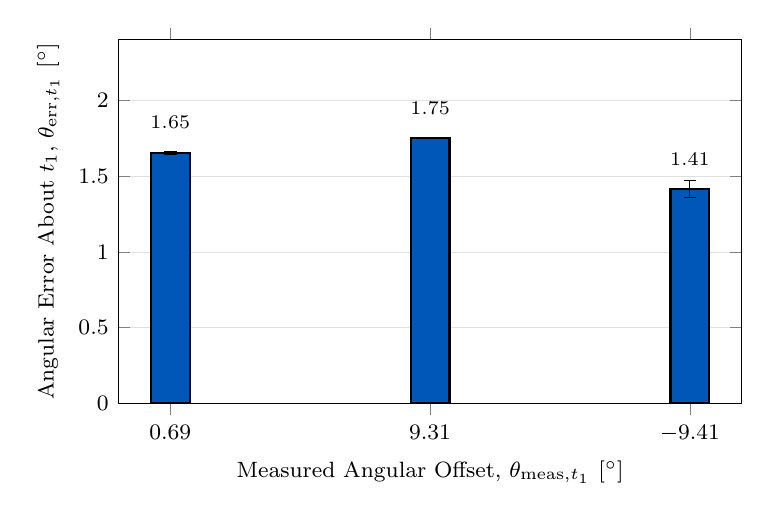
\begin{tikzpicture}
\definecolor{barblue}{HTML}{0057B8}
\begin{axis}[
    width=9.5cm, height=6.2cm,
    ybar, bar width=14pt,
    xtick=data, symbolic x coords={none,p10t1,m10t1},
    xticklabels={\(0.69\), \(9.31\), \(-9.41\)},
    ymin=0, ymax=2.4, ytick={0,0.5,1,1.5,2},
    xlabel={Measured Angular Offset, \(\theta_{\mathrm{meas},t_1}\) [\(^\circ\)]},
    ylabel={Angular Error About \(t_1\), \(\theta_{\mathrm{err},t_1}\) [\(^\circ\)]},
    nodes near coords,
    nodes near coords style={font=\scriptsize, yshift=5pt, /pgf/number format/fixed,
                             /pgf/number format/precision=2},
    ymajorgrids=true, xmajorgrids=false,
    grid style={gray!25, very thin},
    tick label style={font=\footnotesize},
    label style={font=\footnotesize},
    legend style={font=\scriptsize, draw=none, fill=none,
                  cells={anchor=west}, at={(0.5,-0.24)}, anchor=north},
    every axis plot/.append style={thick, mark size=2.3pt},
  ]
\addplot[draw=black, fill=barblue, error bars/.cd, y dir=both, y explicit]
coordinates {
  (none,1.653333333) +- (0,0.011547005)
  (p10t1,1.750000000) +- (0,0.000000000)
  (m10t1,1.413333333) +- (0,0.056862407)};
\end{axis}
\end{tikzpicture}
\end{document}
